In this kind of survey, it is essential to ensure the participants’ diversity to get sufficiently accurate and generally reflective results. The Android developer survey found participants through the author's current and former colleagues working in seven different well-known companies in different parts of the world. Also, as previously stated in section \ref{section:4.1.1}, the survey reached answers from random Android developers through various social media platforms. In this way, the participants’ diversity was increased, and getting more accurate results was ensured. Also, the first question was added to the survey to find out the participant competence. The experience of an Android developer impacts the developer's tendencies when making decisions such as technologies, methods, architectural pattern and so on. Responses gathered from this question can be used to identify such correlations. Results can be seen in Fig. \ref{fig:dev_experience} below.
\begin{figure}[ht!]
    \centering
    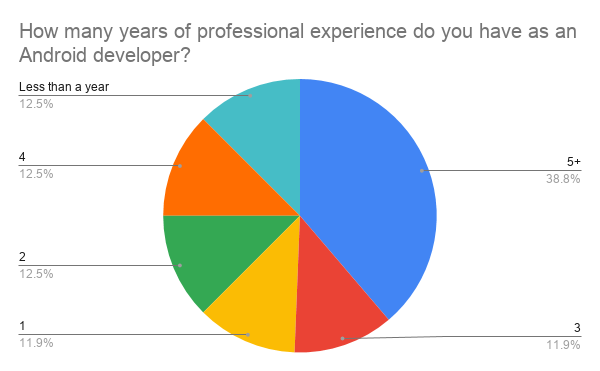
\includegraphics[scale=0.6]{figures/survey_q1_dev_experience.png}
    \caption{Participant background results}
    \label{fig:dev_experience}
\end{figure}
\FloatBarrier
When Fig. \ref{fig:dev_experience} is examined, 63\% of the participants have more than 3 years of experience while around 39\% of them has 5+ years of experience. People with 0-2 years of experience are around 37\% of the all participants.